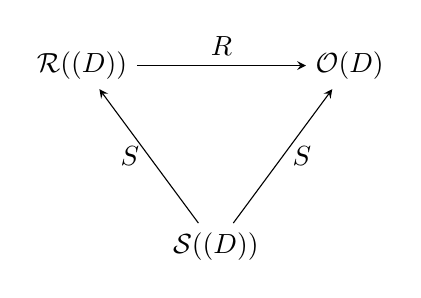
\begin{tikzpicture}

	\node(R1) at (-1.7,0) {$\mathcal{R}(\tc(D))$};
	\node(S1) at (0,-2.3) {$\mathcal{S}(\PP(D))$};
	\node(O1) at (1.7,0) {$\mathcal{O}(D)$};

	\draw[] (R1) edge [-stealth] node [above]{$\orn{R}$}  (O1);

	\draw[] (S1) edge [-stealth] node [left]{$\reori{S}$}  (R1);
	
	\draw[] (S1) edge [-stealth] node [right]{$\orn{S}$}  (O1);
		
	\node at (0,-.9) {\textbf{\huge{$\circlearrowright$}}};

\end{tikzpicture}

\qquad

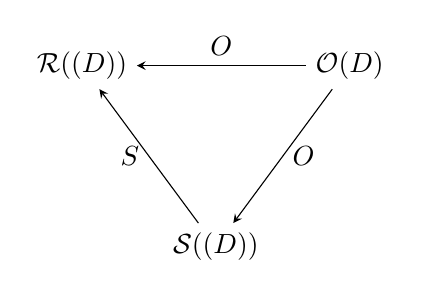
\begin{tikzpicture}

	\node(R2) at (-1.7,0) {$\mathcal{R}(\tc(D))$};
	\node(S2) at (0,-2.3) {$\mathcal{S}(\PP(D))$};
	\node(O2) at (1.7,0) {$\mathcal{O}(D)$};
	
	\draw[] (O2) edge [-stealth] node [above]{$\reori{O}$}  (R2);

	\draw[] (S2) edge [-stealth] node [left]{$\reori{S}$}  (R2);
	
	\draw[] (O2) edge [-stealth] node [right]{$\sour{O}$}  (S2);
		
	\node at (0,-.9) {\textbf{\huge{$\circlearrowright$}}};

\end{tikzpicture}

\qquad

\begin{tikzpicture}

	\node(R3) at (-1.7,0) {$\mathcal{AR}(\tc(D))$};
	\node(S3) at (0,-2.3) {$\mathcal{AS}(\PP(D))$};
	\node(O3) at (1.7,0) {$\mathcal{AO}(D)$};

	\draw[] (R3) edge [-stealth] node [above]{$\orn{R} = \aorn{R}$} (O3);

	\draw[] (R3) edge [-stealth] node [left]{$\asour{R}$} (S3);
		
	\draw[] (S3) edge [-stealth] node [right]{$\orn{S} = \aorn{S}$} (O3);
	
	\node at (0,-.9) {\textbf{\huge{$\circlearrowleft$}}};

\end{tikzpicture}